% Options for packages loaded elsewhere
\PassOptionsToPackage{unicode}{hyperref}
\PassOptionsToPackage{hyphens}{url}
\PassOptionsToPackage{dvipsnames,svgnames,x11names}{xcolor}
\documentclass[
  japanese,
]{ltjsarticle}
\usepackage{xcolor}
\usepackage[margin=25mm]{geometry}
\usepackage{amsmath,amssymb}
\setcounter{secnumdepth}{-\maxdimen} % remove section numbering
\usepackage{iftex}
\ifPDFTeX
  \usepackage[T1]{fontenc}
  \usepackage[utf8]{inputenc}
  \usepackage{textcomp} % provide euro and other symbols
\else % if luatex or xetex
  \usepackage{unicode-math} % this also loads fontspec
  \defaultfontfeatures{Scale=MatchLowercase}
  \defaultfontfeatures[\rmfamily]{Ligatures=TeX,Scale=1}
\fi
\usepackage{lmodern}
\ifPDFTeX\else
  % xetex/luatex font selection
\fi
% Use upquote if available, for straight quotes in verbatim environments
\IfFileExists{upquote.sty}{\usepackage{upquote}}{}
\IfFileExists{microtype.sty}{% use microtype if available
  \usepackage[]{microtype}
  \UseMicrotypeSet[protrusion]{basicmath} % disable protrusion for tt fonts
}{}
\makeatletter
\@ifundefined{KOMAClassName}{% if non-KOMA class
  \IfFileExists{parskip.sty}{%
    \usepackage{parskip}
  }{% else
    \setlength{\parindent}{0pt}
    \setlength{\parskip}{6pt plus 2pt minus 1pt}}
}{% if KOMA class
  \KOMAoptions{parskip=half}}
\makeatother
\usepackage{longtable,booktabs,array}
\newcounter{none} % for unnumbered tables
\usepackage{calc} % for calculating minipage widths
% Correct order of tables after \paragraph or \subparagraph
\usepackage{etoolbox}
\makeatletter
\patchcmd\longtable{\par}{\if@noskipsec\mbox{}\fi\par}{}{}
\makeatother
% Allow footnotes in longtable head/foot
\IfFileExists{footnotehyper.sty}{\usepackage{footnotehyper}}{\usepackage{footnote}}
\makesavenoteenv{longtable}
\usepackage{graphicx}
\makeatletter
\newsavebox\pandoc@box
\newcommand*\pandocbounded[1]{% scales image to fit in text height/width
  \sbox\pandoc@box{#1}%
  \Gscale@div\@tempa{\textheight}{\dimexpr\ht\pandoc@box+\dp\pandoc@box\relax}%
  \Gscale@div\@tempb{\linewidth}{\wd\pandoc@box}%
  \ifdim\@tempb\p@<\@tempa\p@\let\@tempa\@tempb\fi% select the smaller of both
  \ifdim\@tempa\p@<\p@\scalebox{\@tempa}{\usebox\pandoc@box}%
  \else\usebox{\pandoc@box}%
  \fi%
}
% Set default figure placement to htbp
\def\fps@figure{htbp}
\makeatother
\ifLuaTeX
\usepackage[bidi=basic,shorthands=off,provide=*]{babel}
\else
\usepackage[bidi=default,shorthands=off,provide=*]{babel}
\fi
\ifLuaTeX
  \usepackage{selnolig} % disable illegal ligatures
\fi
\setlength{\emergencystretch}{3em} % prevent overfull lines
\providecommand{\tightlist}{%
  \setlength{\itemsep}{0pt}\setlength{\parskip}{0pt}}
\usepackage{bookmark}
\IfFileExists{xurl.sty}{\usepackage{xurl}}{} % add URL line breaks if available
\urlstyle{same}
\hypersetup{
  pdftitle={群衆雑音下のラグビー中継音声からのレフェリー笛検出},
  pdfauthor={野中哲},
  pdflang={ja},
  colorlinks=true,
  linkcolor={blue},
  filecolor={Maroon},
  citecolor={Blue},
  urlcolor={Blue},
  pdfcreator={LaTeX via pandoc}}

\title{群衆雑音下のラグビー中継音声からのレフェリー笛検出}
\usepackage{etoolbox}
\makeatletter
\providecommand{\subtitle}[1]{% add subtitle to \maketitle
  \apptocmd{\@title}{\par {\large #1 \par}}{}{}
}
\makeatother
\subtitle{― エネルギーベース手法の限界と音色ベース分類による打破 ―}
\author{野中哲\thanks{神奈川不惑クラブ}}
\date{2026-06-17}

\begin{document}
\maketitle

\textbf{要旨}

ラグビー試合の中継音声から、レフェリーが吹く笛の時刻を自動検出する課題に取り組んだ。
笛は約2
kHzの狭帯域トーンだが、観客の歓声・チャント・ボールを蹴る音などの強い雑音に
埋もれるため、単純なエネルギー検出では識別が難しい。本研究では、(1)
背景の取り方が
相補的な2つのエネルギーベース検出器とその合議アンサンブル、(2)
候補のスペクトログラムから
音色特徴を抽出して笛/非笛を判別するロジスティック回帰分類器、(3)
検出器の候補だけを
効率的にラベル付けする支援ツール、を構築した。1試合(前半)を全編人手でラベル付けして
得た笛47個を正解とすると、エネルギーベースのアンサンブルは適合率・再現率の調和平均
F1で約56\%が上限であった。一方、音色特徴(立ち上がりの鋭さ・倍音比・低域比など)を
用いた分類器で候補を再ランクすると、5分割交差検証で\textbf{F1は56\%から72\%}へ向上した。
さらに前半で学習した分類器を未学習の後半に適用したところ、後半でも\textbf{F1
74\%→91\%}と
汎化した。本稿は手法・実験・知見を報告するとともに、「音の大小」では分離できない笛を
「音色」で分離するという、人間の聴覚に着想を得た設計指針を示す。

\textbf{キーワード}: 音響イベント検出, スペクトログラム, 笛検出,
アンサンブル, 音色分類, 弱教師

\begin{center}\rule{0.5\linewidth}{0.5pt}\end{center}

\subsection{1. はじめに}\label{ux306fux3058ux3081ux306b}

スポーツ映像の自動編集・ハイライト生成では、試合の節目を示すイベント時刻の取得が重要で
ある。ラグビーにおいてレフェリーの笛は反則・得点・前後半の開始終了など多くの局面を
標識する有力な手がかりとなる。しかし中継音声中の笛は、

\begin{itemize}
\tightlist
\item
  観客の歓声・ざわめき(広帯域・非定常)
\item
  チャント・声援(調波構造をもつ)
\item
  ボールを蹴る音・拍手(瞬発的)
\end{itemize}

といった強い背景音に埋もれる。特に主審がマイクから遠い場面や観客が盛り上がる場面では、
笛のエネルギーが背景と同程度になり、振幅情報だけでは識別が困難になる。

本研究の貢献は次の通りである。

\begin{enumerate}
\def\labelenumi{\arabic{enumi}.}
\tightlist
\item
  背景推定の異なる2つのエネルギーベース検出器と、その合議によるアンサンブルを設計した。
\item
  エネルギーベース手法がF1 ≈
  56\%で頭打ちになることと、その原理的理由を実測で示した。
\item
  スペクトログラムから抽出した音色特徴による分類器で候補を再ランクし、頭打ちを打破した
  (交差検証 F1 56→72\%)。さらに別ハーフへの汎化(F1 74→91\%)を確認した。
\item
  音声領域の前処理(調波・打楽器分離;
  HPSS)は本課題では有効でないという否定的結果を 実測で示した。
\item
  検出器の候補だけを音声+スペクトログラム付きでレビューし高速にラベル付けする支援
  ツールを構築し、ラベリングにおける実践的知見(クリップはエネルギーピークに中心を
  合わせるべき)を得た。
\end{enumerate}

\subsection{2. データ}\label{ux30c7ux30fcux30bf}

公式リーグ戦1試合の中継動画を用いた。音声は48 kHz・モノラル・16 bit
PCMに変換した。

{\def\LTcaptype{none} % do not increment counter
\begin{longtable}[]{@{}
  >{\raggedright\arraybackslash}p{(\linewidth - 6\tabcolsep) * \real{0.2667}}
  >{\raggedright\arraybackslash}p{(\linewidth - 6\tabcolsep) * \real{0.2000}}
  >{\raggedright\arraybackslash}p{(\linewidth - 6\tabcolsep) * \real{0.3333}}
  >{\raggedright\arraybackslash}p{(\linewidth - 6\tabcolsep) * \real{0.2000}}@{}}
\toprule\noalign{}
\begin{minipage}[b]{\linewidth}\raggedright
ハーフ
\end{minipage} & \begin{minipage}[b]{\linewidth}\raggedright
長さ
\end{minipage} & \begin{minipage}[b]{\linewidth}\raggedright
笛(正解)
\end{minipage} & \begin{minipage}[b]{\linewidth}\raggedright
備考
\end{minipage} \\
\midrule\noalign{}
\endhead
\bottomrule\noalign{}
\endlastfoot
前半 & 44分10秒 (2647 s) & 47 & 全編リスニングでラベル付け \\
後半 & 47分28秒 (2848 s) & 41(候補中) &
検出器候補をレビューでラベル付け \\
\end{longtable}
}

前半は人手で全編を聴いて笛を書き起こした。当初48個と記録したが、後述するクリップ
精査により1個が数え過ぎと判明し、最終的に\textbf{笛47個}とした。加えて、検出器が誤検出
しやすい「笛でない強いトーン」2個(例: 29:55)をハード負例として記録した。

後半は本研究で構築した支援ツールにより、検出器が出した候補118個をレビューして
\textbf{笛41 /
非笛77}に分類した。後半は全編リスニングを行っていないため、後半の正解は
「候補に含まれる笛」に限られる(2.の限界として後述)。

\subsection{3. 手法}\label{ux624bux6cd5}

\subsubsection{3.1
エネルギーベース検出}\label{ux30a8ux30cdux30ebux30aeux30fcux30d9ux30fcux30b9ux691cux51fa}

笛は基本波 f0 ≈ 1.7--2.5 kHz
とその倍音をもつ、短いが持続的な狭帯域トーンである。
音声をSTFTでスペクトログラム化し、フレームごとに以下を評価して笛らしさを数値化する。

\begin{itemize}
\tightlist
\item
  \textbf{トーン性}: 笛帯域でのピークエネルギーの集中度(ピーク/帯域和)
\item
  \textbf{倍音の同時性}: f0 と 2f0 帯域のエネルギーの同時の強さ
\item
  \textbf{背景に対するコントラスト}: ピークを背景レベルで割った突出度
\item
  \textbf{持続}: 一定時間トーンが続くか(瞬発音の除去)
\end{itemize}

背景レベルの取り方を変えた2つの「専門家」を用意した。

\begin{itemize}
\tightlist
\item
  \textbf{v1}: 12
  kHzにダウンサンプルし、コントラストの分母に\textbf{低域(150--1300
  Hz)の群衆レベル}を
  用いる。持続をやや長めに要求する。明瞭で持続的な笛に強い(高精度)が、短い笛や群衆が
  大きい場面の弱い笛を取り逃す。
\item
  \textbf{v2}: 24
  kHzで解析し、コントラストの分母に\textbf{笛帯域そのものの時間方向の局所背景}を用いる。
  持続要求を短くする。人間の聴覚の周波数選択性(低域の群衆は2
  kHzの笛をマスクしない)を
  反映し、短い/弱い笛を拾えるが、瞬発的な縦縞ノイズ等の誤検出が増える。
\end{itemize}

各検出器はフレームスコアの局所ピークをイベント化して候補を出す。両者の候補を、各検出器
での「(候補数の上限 −
順位)」を加算した\textbf{合議スコア}でグローバルに再ランクする
(両方に出る候補ほど高信頼)。これを本番の候補生成器(アンサンブル)とする。

\subsubsection{3.2
評価方法と正解データ}\label{ux8a55ux4fa1ux65b9ux6cd5ux3068ux6b63ux89e3ux30c7ux30fcux30bf}

検出時刻が正解の笛時刻と±4
s以内で一致すれば真陽性(TP)とする貪欲1対1照合を用い、
上位N件を採ったときの適合率(precision)・再現率(recall)・F1を曲線として評価する。
あわせて、候補中に含まれる正解笛の割合を\textbf{再現率上限}と定義する(候補に無い笛は
どんな再ランクでも拾えないため)。

\subsubsection{3.3 前処理の検討:
HPSS(否定的結果)}\label{ux524dux51e6ux7406ux306eux691cux8a0e-hpssux5426ux5b9aux7684ux7d50ux679c}

スペクトログラムを時間方向メディアン(調波=笛)と周波数方向メディアン(打楽器=ボール音)に
分離し、調波成分を強調した音声を再構成して検出器に入力した。しかし2通りのカーネル設定の
いずれでも、\textbf{再現率上限が悪化し(90\%→69〜77\%)、F1は改善しなかった}。原因は、
(i) 音声再構成(逆STFT)が弱い笛を損なうこと、(ii)
v2が既に帯域内の局所背景比で適応
正規化しており前処理と重複すること、(iii)
声・チャントも調波構造をもつため笛と分離
できないこと、である。よって本課題では音声領域の前処理は採用しない。

\subsubsection{3.4
音色ベース分類器}\label{ux97f3ux8272ux30d9ux30fcux30b9ux5206ux985eux5668}

エネルギーベースの頭打ちを打破するため、候補のスペクトログラム(±0.4
s窓)から音色特徴
11次元を抽出し、笛/非笛をロジスティック回帰で判別して候補を再ランクする。特徴は
突出度・トーン性・倍音比(f0,2f0,3f0)・ピッチ安定性・低域比・高域比・持続・立ち上がりの
鋭さ・スペクトル平坦度などである。学習は標準化+L2正則化、評価は5分割交差検証の
out-of-foldスコアで行い、学習データへの過適合を排した。

\subsubsection{3.5
教師データ作成支援ツール}\label{ux6559ux5e2bux30c7ux30fcux30bfux4f5cux6210ux652fux63f4ux30c4ux30fcux30eb}

別試合のラベル付けを効率化するため、検出器の候補(高再現)だけをレビューする自己完結
HTMLを生成するツールを構築した。各候補に音声クリップとスペクトログラムを埋め込み、
キーボードで笛/非笛/保留を高速にラベル付けできる。ローカルサーバへの自動保存により
書き出し操作を不要にし、進捗ミニマップ・未/済の色分け・未ラベルへのジャンプを備える。
重要な改良として、レビュー用クリップを候補時刻ではなく\textbf{近傍の笛帯域エネルギーピークに
中心を合わせ直す}処理を導入した(3.5の知見、4.4)。

\subsection{4. 実験結果}\label{ux5b9fux9a13ux7d50ux679c}

\subsubsection{4.1 検出器の性能(前半,
笛47)}\label{ux691cux51faux5668ux306eux6027ux80fdux524dux534a-ux7b1b47}

各検出器の再現率上限と、アンサンブル合議ランキングの動作点を表に示す。

{\def\LTcaptype{none} % do not increment counter
\begin{longtable}[]{@{}ll@{}}
\toprule\noalign{}
検出器 & 再現率上限 \\
\midrule\noalign{}
\endhead
\bottomrule\noalign{}
\endlastfoot
v1 単独 & 58\% \\
v2 単独 & 79\% \\
アンサンブル(v1∪v2) & \textbf{約90\%} \\
\end{longtable}
}

{\def\LTcaptype{none} % do not increment counter
\begin{longtable}[]{@{}llll@{}}
\toprule\noalign{}
N(上位件数) & precision & recall & F1 \\
\midrule\noalign{}
\endhead
\bottomrule\noalign{}
\endlastfoot
15 & 100\% & 31\% & 48\% \\
30 & 73\% & 46\% & \textbf{56\%(最良)} \\
70 & 44\% & 65\% & 53\% \\
120 & 36\% & 90\% & 51\% \\
\end{longtable}
}

上位15件は誤検出ゼロである一方、F1は約56\%で頭打ちとなる。再現率上限は約90\%で、
\textbf{残り4個の笛(1:57, 11:35, 12:39,
23:57)はどの設定でも候補に上がらない}。これらは
背景に対する帯域内突出が小さく(例:
1:57は突出1.7倍。検出可能な笛は3〜6倍)、
エネルギー情報だけでは背景と分離できない。

\subsubsection{4.2 前処理(HPSS)}\label{ux524dux51e6ux7406hpss}

{\def\LTcaptype{none} % do not increment counter
\begin{longtable}[]{@{}lll@{}}
\toprule\noalign{}
入力 & 再現率上限 & F1最良 \\
\midrule\noalign{}
\endhead
\bottomrule\noalign{}
\endlastfoot
前処理なし & 90\% & 56\% \\
HPSS (KT=7,KF=9) & 69\% & 58\% \\
HPSS (KT=3,KF=13) & 77\% & 56\% \\
\end{longtable}
}

前処理は再現率上限をむしろ下げ、F1を改善しなかった(3.3)。

\subsubsection{4.3 音色分類器(前半,
5分割交差検証)}\label{ux97f3ux8272ux5206ux985eux5668ux524dux534a-5ux5206ux5272ux4ea4ux5deeux691cux8a3c}

{\def\LTcaptype{none} % do not increment counter
\begin{longtable}[]{@{}lll@{}}
\toprule\noalign{}
N & baseline P/R/F1 & 分類器 P/R/F1 \\
\midrule\noalign{}
\endhead
\bottomrule\noalign{}
\endlastfoot
30 & 73 / 46 / 56 & \textbf{90 / 56 / 69} \\
40 & 57 / 48 / 52 & \textbf{78 / 65 / 70} \\
最良 & \textbf{56\%} & \textbf{72\%} \\
\end{longtable}
}

\textbf{F1は56\%→72\%(+16ポイント)}に向上した(図1,
図2)。回帰係数の大きい特徴は、立ち上がりの 鋭さ(onset,
最大の正係数)、低域比(群衆の少なさ,
負係数)、倍音比、持続であり(図3)、「笛らしい
音色」を学習していることを示す。再現率上限は候補集合に依存するため90\%のままで、分類器は
あくまで既存候補の\textbf{ランキング品質}を改善する。

\begin{figure}
\centering
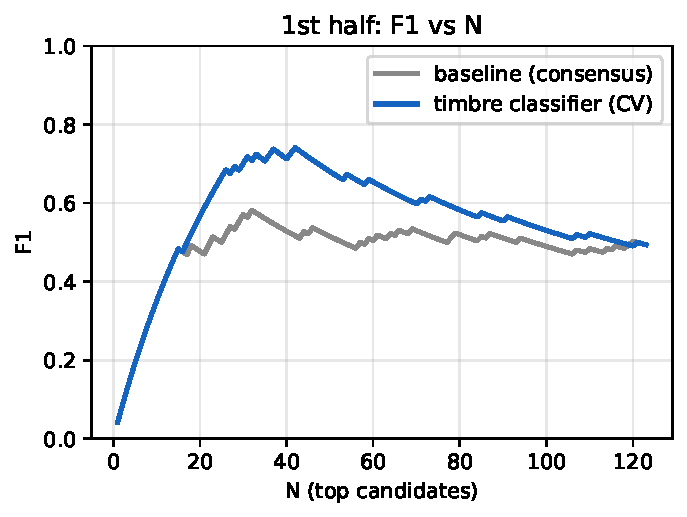
\includegraphics[width=0.68\linewidth,height=\textheight,keepaspectratio,alt={前半におけるF1の比較。合議スコア順(baseline)に対し、音色分類器(交差検証)はあらゆる上位N件でF1が高い。}]{figs/fig1_f1_1st.pdf}
\caption{前半におけるF1の比較。合議スコア順(baseline)に対し、音色分類器(交差検証)はあらゆる上位N件でF1が高い。}
\end{figure}

\begin{figure}
\centering
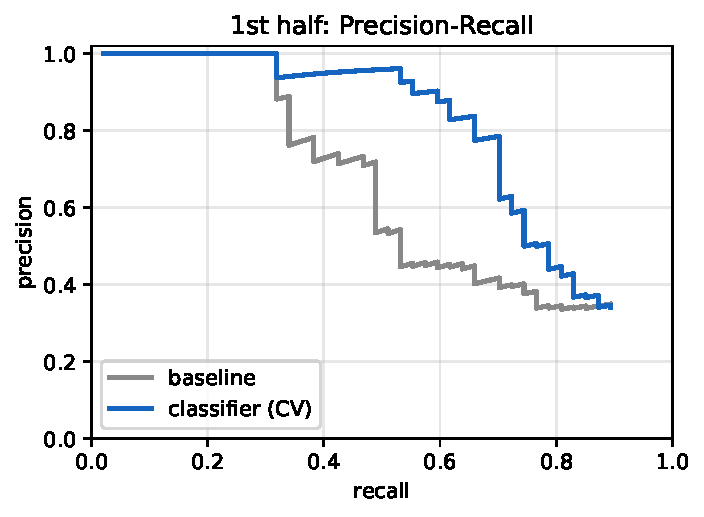
\includegraphics[width=0.68\linewidth,height=\textheight,keepaspectratio,alt={前半の適合率--再現率曲線。分類器(交差検証)はbaselineを一貫して上回る。}]{figs/fig2_pr_1st.pdf}
\caption{前半の適合率--再現率曲線。分類器(交差検証)はbaselineを一貫して上回る。}
\end{figure}

\begin{figure}
\centering
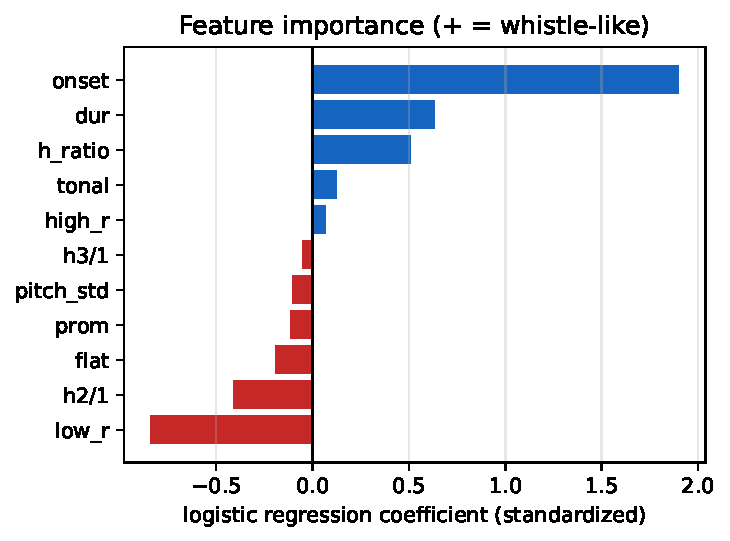
\includegraphics[width=0.68\linewidth,height=\textheight,keepaspectratio,alt={ロジスティック回帰の標準化係数。立ち上がりの鋭さ(onset)が最も笛らしさに寄与し、低域比(low\_r=群衆の大きさ)は負に効く。}]{figs/fig4_coef.pdf}
\caption{ロジスティック回帰の標準化係数。立ち上がりの鋭さ(onset)が最も笛らしさに寄与し、低域比(low\_r=群衆の大きさ)は負に効く。}
\end{figure}

\subsubsection{4.4 汎化:
前半で学習→後半でテスト}\label{ux6c4eux5316-ux524dux534aux3067ux5b66ux7fd2ux5f8cux534aux3067ux30c6ux30b9ux30c8}

前半の笛で学習した分類器を、未学習の後半候補(笛41/非笛77)に適用した。

{\def\LTcaptype{none} % do not increment counter
\begin{longtable}[]{@{}llll@{}}
\toprule\noalign{}
後半での手法 & precision & recall & F1 \\
\midrule\noalign{}
\endhead
\bottomrule\noalign{}
\endlastfoot
baseline(合議スコア順) & 75\% & 73\% & 74\% \\
分類器(前半で学習→後半に適用) & \textbf{92\%} & \textbf{90\%} &
\textbf{91\%} \\
\end{longtable}
}

\textbf{F1
74\%→91\%}。音色特徴が試合(ハーフ)をまたいで有効であることを示す(図4)。

\begin{figure}
\centering
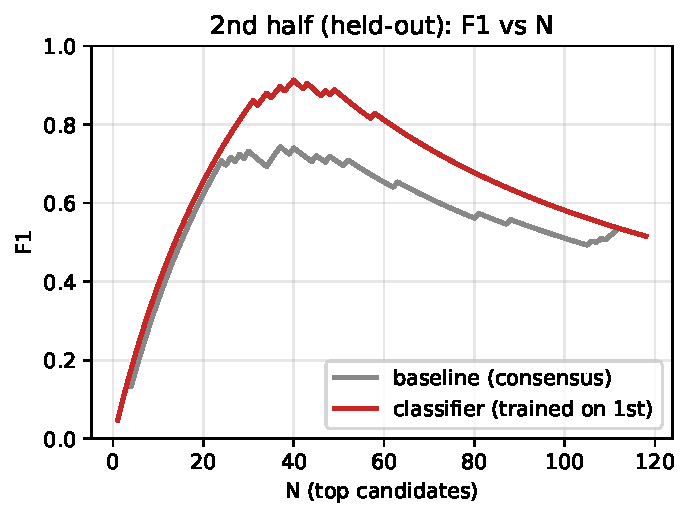
\includegraphics[width=0.68\linewidth,height=\textheight,keepaspectratio,alt={後半(未学習データ)でのF1。前半で学習した分類器がbaselineを上回り、F1は74\%→91\%に向上する。}]{figs/fig3_generalize.pdf}
\caption{後半(未学習データ)でのF1。前半で学習した分類器がbaselineを上回り、F1は74\%→91\%に向上する。}
\end{figure}

加えて、支援ツールの設計に関する知見を得た。候補だけのレビューでは前半の笛が30個しか
拾えず、全編リスニングの47個と13個食い違った。その13個を「正解時刻に中心を合わせた
クリップ」で聴き直すと\textbf{12個は笛}であった。原因は候補の時刻が実際の笛と数秒ずれ、
候補中心のクリップが笛を外していたことである。残り1個は数え過ぎであった。この知見から、
レビュー用クリップを近傍のエネルギーピークに中心合わせする処理を導入した(3.5)。

\subsection{5. 考察}\label{ux8003ux5bdf}

\subsubsection{5.1
なぜエネルギーでは頭打ちか}\label{ux306aux305cux30a8ux30cdux30ebux30aeux30fcux3067ux306fux982dux6253ux3061ux304b}

エネルギーベース手法は「笛帯域がどれだけ大きく突出したか」を測る。しかし観客の声や
チャントは笛と同程度の音量・同様の調波構造をもつため、振幅・突出度だけでは笛と分離
できない。これがF1 ≈ 56\%の壁の本質である。

\subsubsection{5.2
人間の聴覚との対応}\label{ux4ebaux9593ux306eux8074ux899aux3068ux306eux5bfeux5fdc}

人間は群衆が大きい場面でも1:57の弱い笛を明瞭に聞き取る。これは振幅比ではなく、
(i) 周波数選択性(臨界帯域: 低域の群衆は2 kHzの笛をマスクしない)、(ii)
倍音のグループ化 (聴覚情景分析)、(iii)
立ち上がり・時間微細構造への鋭敏さ、(iv) 音色・パターンの認識、に
よる。本研究のv2は(i)を、音色分類器は(iv)を計算的に近似したものと位置づけられる。
立ち上がり(onset)が分類の最重要特徴であった点は(iii)とも整合する。

\subsubsection{5.3 限界}\label{ux9650ux754c}

\begin{itemize}
\tightlist
\item
  検出不能な4個の笛は候補に上がらないため、分類器でも回収できない。候補生成器(検出器)の
  感度向上が別途必要である。
\item
  前半/後半は同一試合(同じ主審・笛・録音環境)であり、別主審・別会場・別放送への汎化は
  未検証である。
\item
  後半の正解は候補ベースであり、全編リスニングを行っていないため後半の絶対再現率は
  未確定である。報告した汎化はランキング品質の改善である。
\end{itemize}

\subsection{6. 結論と今後}\label{ux7d50ux8ad6ux3068ux4ecaux5f8c}

群衆雑音下の笛検出において、エネルギーベース手法はF1 ≈
56\%で頭打ちになること、そして
音色ベースの分類器がこの壁を打破し(交差検証 F1
72\%)、別ハーフへ汎化する(F1 91\%)ことを
実測で示した。否定的結果として、音声領域のHPSS前処理は本課題で有効でないことも示した。
今後は、(1)
分類器を本番パイプラインへ組み込み(モデル保存→新規試合へ適用)、(2)
複数試合・ 複数会場のデータによる真の汎化検証、(3)
検出不能な弱い笛を拾うための候補生成器の改良、 (4)
全編リスニングによる絶対再現率の確立、に取り組む。

\subsection{付録: 再現性}\label{ux4ed8ux9332-ux518dux73feux6027}

本研究の実装は単一リポジトリ \url{https://github.com/anonaka/fue}
にまとめ、Python(numpy)と ffmpeg/ffprobeのみで動作する。
主なスクリプトは、検出器(\texttt{detect\_whistle.py}, \texttt{\_v1.py},
\texttt{\_v2.py})、評価(\texttt{evaluate.py})、
音色分類器(\texttt{classify.py}, 汎化検証
\texttt{classify\_generalize.py})、前処理実験(\texttt{preprocess.py})、
ラベル付け支援(\texttt{make\_review.py},
\texttt{review\_server.py})、マーカー生成(\texttt{make\_chapters.py})である。
正解データは \texttt{labels/ground\_truth.tsv}(前半),
\texttt{labels/ground\_truth\_2nd.tsv}(後半)に TSV形式で保持する。

\end{document}
